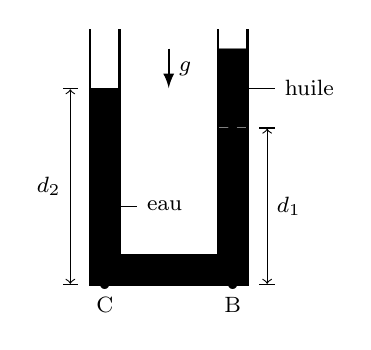
\begin{tikzpicture} [
	scale=.5,
	font=\footnotesize,
	vecteur/.style={-latex,thick},
	liquide/.style={fill=\JRLblueC,very thin,draw=\JRLblueF},
	huile/.style={fill=\JRLyellow,very thin,draw=gray},
	]
%	\shadedraw[color=gray,top color=white,bottom color=gray] (-2,5)--++(0,-5)--++(4,0)--++(0,4)--++(-0.5,0)--++(0,-3.5)--++(-3,0)--++(0,4.5) --cycle;
	\draw[liquide] (-2,5)--++(0,-5)--++(4,0)--++(0,4)--++(-0.75,0)--++(0,-3.25)--++(-2.5,0)--++(0,4.25) --cycle;
	 \draw[huile] (2,4)--++(0,2)--++(-0.75,0)--++(0,-2) --cycle;
	 \draw[line width=1pt] (-2,6.5)--++(0,-6.5)--++(4,0)--++(0,6.5);
	 \draw[line width=1pt] (-1.25,6.5)--++(0,-5.75)--++(2.5,0)--++(0,5.75);
	 \draw[vecteur] (0,6)--++(0,-1) node[pos=0.5,right]{$\vv{g}$};
	 \draw[<-] (1.7,5)--++(1,0) node[right]{huile};
	 \draw[<-] (-1.8,2)--++(1,0) node[right]{eau};
	 \draw[|<->|,shift={(2.5,4)}] (0,0)--++(0,-4)node[midway,right]{\(d_1\)};
	 \draw[|<->|,shift={(-2.5,5)}] (0,0)--++(0,-5)node[midway,left]{\(d_2\)};
	 % points
	 \draw[shift={(1.625,4)}] (0,0) node{$\bullet$}node[below=1pt]{A};	 
	 \draw[shift={(1.625,0)}] (0,0) node{$\bullet$}node[below=1pt]{B};	 
	 \draw[shift={(-1.625,0)}] (0,0) node{$\bullet$}node[below=1pt]{C};	 
 \end{tikzpicture}
